\documentclass[12pt,a4paper]{beamer}
\usepackage[utf8]{inputenc}
\usepackage[T1]{fontenc}
\usepackage{amsmath}
\usepackage{amsfonts}
\usepackage{amssymb}
\usepackage{graphicx}
\usepackage[portuguese]{babel}
\usepackage{amsthm}
\usepackage{amsmath}
\usepackage[alf]{abntex2cite}
\usepackage{parskip}

\usetheme{Madrid}

\author{Mario Alexis Lamas Espinoza \\ Orientador: Prof. Dr. Fernando Manfio}
\title{Superfícies Mínimas e a Conjectura de Lawson}
\setbeamertemplate{theorems}[numbered]

\newtheorem{teorema}{Teorema}
\newtheorem{proposicao}{Proposição}
\theoremstyle{definition}
\newtheorem{definicao}{Definição}
\newtheorem{observacao}{Observação}
\newtheorem{exemplo}{Exemplo}
\newtheorem{corolario}{Corolário}


\newcommand{\vectorfieldsspace}[1]{
	\mathfrak{X}(#1)
}

\newcommand{\normalvectorfieldsspace}[1]{
	\mathfrak{N}(#1)
}

\newcommand{\smoothfunctionsspace}[1]{
	C^\infty(#1)
}

\newcommand{\innerproduct}[2]{
	\left\langle #1,#2 \right\rangle
}

\newcommand{\realnumbers}{
	\mathbb{R}
}


\newcommand{\xb}{
	\overline{x}	
}



\newcommand{\yb}{
	\overline{y}	
}

\newcommand{\R}{\mathbb R}
\newcommand{\Sp}{\mathbb{S}}


\newcommand{\pdiff}[1]{
	\frac{\partial}{\partial #1}
}



\newcommand{\partialdiff}[2]{\frac{\partial #1}{\partial #2}}

\newcommand{\npartialdifffrac}[3]{\frac{\partial^#3 #1}{\partial #2^#3}}





\newcommand{\liebrackets}[2]{
	\left[ #1, #2 \right]
}



\newcommand{\curvaturetensor}[3]{
	\mathcal{R} \left( #1,#2 \right) #3
}

\newcommand{\norm}[1]{
	\left| #1 \right|
}


\newcommand{\complexnumbers}{
	\mathbb{C}
}

\newcommand{\N}{
	\mathbb{N}
}

\newcommand{\euclideanconnection}{
	\overline{\nabla}
}

\newcommand{\tangentialconnection} {
	\nabla^\top
}

\newcommand{\parentheses}[1]{
	\left( #1 \right)
}

\DeclareMathOperator\supp{supp}

\begin{document}

\begin{frame}
	\maketitle	
\end{frame}

\section{Superfícies Mínimas}

\begin{frame}
	\frametitle{Superfícies Mínimas}
	\begin{definicao}
		Dado uma imersão isométrica $f: M \rightarrow \tilde{M}$, seja $f^* T\tilde{M}$ o fibrado induzido sobre $M$, cuja fibra em $p \in M$ é $T_{f(p)} \tilde{M}$. O complemento ortogonal de $f_* T_p M$ em $T_{f(p)} \tilde{M}$, denotado por $T_p M^\perp$, chama-se o \emph{espaço normal} de $f$ em $p$. O fibrado normal $TM^\perp$ de $f$ é o subfibrado vetorial de $f^* T \tilde{M}$, cuja fibra em $p \in M$ é $T_p M^\perp$.  
	\end{definicao}
\end{frame}

\begin{frame}
	A conexão Levi-Civita $\tilde{\nabla}$ de $\tilde{M}$ induz uma única conexão $\hat{\nabla}$ em $f^* T \tilde{M}$ tal que
	\begin{equation*}
		\hat{\nabla}_X (Z \circ f) = \tilde{\nabla}_{f_* X} Z, 
	\end{equation*}
	para quaisquer $X \in \vectorfieldsspace{M}$ e $Z \in \vectorfieldsspace{M}$. Identificaremos sempre $\hat{\nabla}$ com $\tilde{\nabla}$.
	
	Dados dois campos $X,Y \in \vectorfieldsspace{M}$, decompomos
	\begin{equation*}
		\tilde{\nabla}_X f_* Y = \parentheses{\tilde{\nabla}_X f_* Y}^\top + \parentheses{\tilde{\nabla}_X f_* Y}^\perp,
	\end{equation*}  
	em relação à descomposição ortogonal
	\begin{equation*}
		f^* T \tilde{M} = f_* TM \oplus TM^\perp.
	\end{equation*}
\end{frame}


\begin{frame}
	A aplicação
	\begin{equation*}
	\nabla_X Y = f_*^{-1} \parentheses{\tilde{\nabla}_X f_* Y}^\top
	\end{equation*}
	define uma conexão compatível e sem torção em $TM$, logo coincide com a conexão Levi-Civita de $M$.
	
	\begin{definicao}
		A aplicação $\alpha_f: \vectorfieldsspace{M} \times \vectorfieldsspace{M} \rightarrow \Gamma(TM^\perp)$ definida por
		\begin{equation*}
			\alpha_f(X,Y) = \parentheses{\tilde{\nabla}_X f_* Y}^\perp,
		\end{equation*}
		chama-se de \emph{segunda forma fundamental} da imersão isométrica $f$.
	\end{definicao}
\end{frame}

\begin{frame}
	\begin{definicao}
		O \emph{vetor curvatura média} de $f$ no ponto $p \in M$ é o vetor normal
		\begin{equation}\label{vetor-curvatura-media}
			H(p) = \frac{1}{m} \sum_{i=1}^m \alpha_f(X_i,X_i),
		\end{equation}
		onde $\{X_1, \ldots, X_m \}$ é uma base ortonormal de $T_p M$. Segue de \eqref{vetor-curvatura-media} que
		\begin{align*}
			m \innerproduct{H}{\xi} &= \sum_{i=1}^m \innerproduct{\alpha_f(X_i,X_i)}{\xi} = \sum_{i=1}^m \innerproduct{A_{\xi} X_i}{X_i}\\
			&= \tr A_{\xi},
		\end{align*}
		logo o lado direito de \eqref{vetor-curvatura-media} não depende da escolha da base ortonormal.
	\end{definicao}
\end{frame}

\begin{frame}
	\begin{definicao}
		Uma imersão isométrica $f: M \rightarrow \tilde{M}$ é dita ser \emph{mínima no ponto} $p \in M$ se $H(p)=0$. Diremos que $f$ é \emph{mínima} se for mínima em todos os pontos $p \in M$.
	\end{definicao}

	\begin{observacao}
		Em particular, em $\R^3$, o vetor curvatura média de uma superfície é un escalar e está definido por
		\begin{equation*}
			H(p) = \frac{1}{2} \parentheses{k_1 + k_2},
		\end{equation*}
		onde $k_1,k_2$ são as curvaturas principais.
	\end{observacao}
\end{frame}

\begin{frame}
	\begin{definicao}
		Dada uma superfície regular $M$ em $\R^3$, uma \emph{carta local isoterma} $(U, \varphi)$ de $M$ é carta local que satisfaz
		\begin{equation*}
			E = G = \lambda^2 \quad \text{e} \quad F=0,
		\end{equation*}
		onde $\lambda: U \rightarrow \R$ é uma função diferenciável, com $\lambda > 0$.
	\end{definicao}
	
	\begin{definicao}
		Seja $(U, \varphi)$ uma carta local para $M$, como $\varphi = \parentheses{\varphi_1, \varphi_2, \varphi_3}$, definimos
		\begin{equation*}
			\Delta \varphi = \parentheses{\Delta \varphi_1, \Delta \varphi_2, \Delta \varphi_3}.
		\end{equation*}
	\end{definicao}
	
\end{frame}

\begin{frame}
	\begin{definicao}
		Uma carta local $(U,\varphi)$ é harmônica se, e somente se,
		\begin{equation*}
			\Delta \varphi \equiv 0.
		\end{equation*}
	\end{definicao}
	
	\begin{corolario}
		Uma superfície $M$ em $\R^3$ é mínima se, e somente se, toda carta local isoterma é harmônica.
	\end{corolario}
\end{frame}

\begin{frame}
	\begin{exemplo}
		O \emph{catenoide} é uma superfície mínima em $\R^3$ parametrizada por
		\begin{equation*}
			\varphi(u,v) = \parentheses{a \cosh v \cos u, a \cosh v \sin u, a v},
		\end{equation*}
		onde  $u \in \parentheses{0, 2\pi}$ e $v \in \R$.
	\end{exemplo}

	Neste exemplo temos
	\begin{equation*}
		E = G = a^2 \cosh^2 v, \quad F = 0 \quad \text{e} \quad \Delta \varphi \equiv 0.
	\end{equation*}
\end{frame}

\begin{frame}
	\begin{figure}
		\centering
		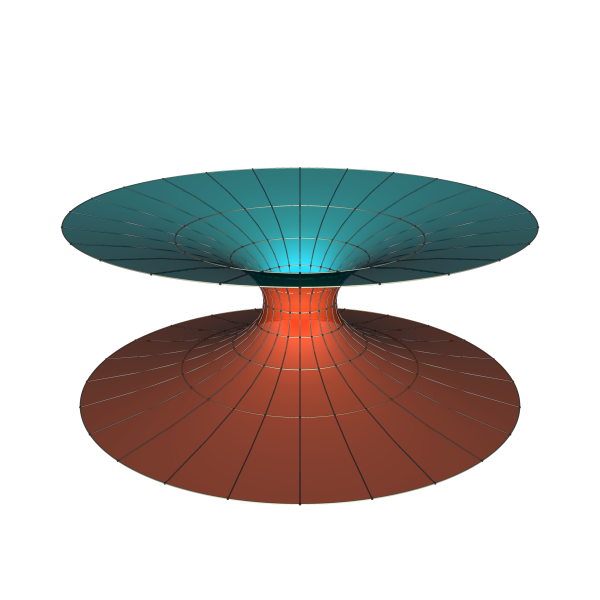
\includegraphics[width=0.5\textwidth]{images/catenoid}
		\caption{Catenoide. Autor: Matthias Weber. Licencia: Creative Commons Attribution-Noncommercial-No Derivative Works 3.0 Unported License (\url{http://creativecommons.org/licenses/by-nc-nd/3.0/}). Enlace: \url{https://minimal.sitehost.iu.edu/archive/Classical/Classical/Catenoid/web/index.html}}
	\end{figure}
\end{frame}

\begin{frame}
	\begin{exemplo}
		O \emph{helicoide} é uma superfície mínima em $\R^3$ parametrizada por
		\begin{equation*}
			\varphi(u,v) = \parentheses{a \sinh v \cos u, a \sinh v \sin u, au},
		\end{equation*}
		onde $u \in \parentheses{0, 2\pi}$ e $v \in \R$.
	\end{exemplo}
	Neste exemplo temos
	\begin{equation*}
		E = G = a^2 \cosh^2 v, \quad F = 0 \quad \text{e} \quad \Delta \varphi \equiv 0.
	\end{equation*}
\end{frame}

\begin{frame}
	\begin{figure}
		\centering
		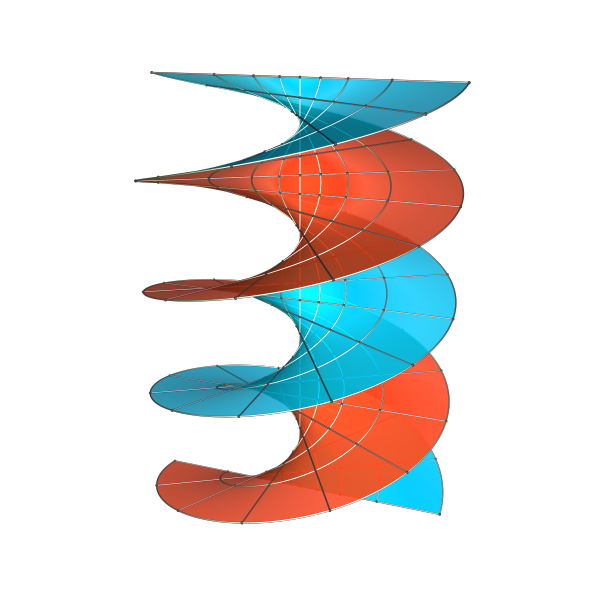
\includegraphics[width=0.5\textwidth]{images/helicoid}
		\caption{Helicoide. Autor: Matthias Weber. Licencia: Creative Commons Attribution-Noncommercial-No Derivative Works 3.0 Unported License (\url{http://creativecommons.org/licenses/by-nc-nd/3.0/}). Enlace: \url{https://minimal.sitehost.iu.edu/archive/Classical/Classical/Helicoid/web/index.html}}
	\end{figure}
\end{frame}

\begin{frame}
	\begin{proposicao}
		Não existem superfícies mínimas fechadas em $\R^3$.
	\end{proposicao}

	\begin{observacao}
		Em $\Sp^3$ existem superfícies mínimas fechadas.
	\end{observacao}
\end{frame}


\begin{frame}
	\begin{exemplo}
		A superfície fechada em $\Sp^3$ definida por
		\begin{equation*}
			M = \{ x \in \Sp^3 \subset \R^4: x_4 = 0 \},
		\end{equation*}
		é chamada de \emph{equador} e é uma superfície mínima porque ambas curvaturas principais são iguais a zero.
	\end{exemplo}
\end{frame}



\begin{frame}
	%\frametitle{Toro de Clifford}
	
	Outro exemplo de uma superfície fechada em $\Sp^3$ que é mínima é o \emph{toro de Clifford}.
	
	\begin{definicao}
		Seja $f: \R^2 \rightarrow S^3$ definida por
		\begin{equation*}
			f(u,v) = \frac{1}{\sqrt{2}} \left(\cos u, \sin u, \cos v, \sin v\right).
		\end{equation*}
		$f$ é chamada de \emph{toro de Clifford}.
	\end{definicao}

	\begin{observacao}
		$f$ é um toro porque é congruente com $S^1 \left(\frac{1}{\sqrt{2}}\right) \times S^1 \left(\frac{1}{\sqrt{2}}\right)$.
	\end{observacao}
\end{frame}

\begin{frame}
	\begin{observacao}
		Por muito tempo o equador e o toro de Clifford eram os únicos exemplos de superfícies mínimas mergulhadas em $\Sp^3$. No entanto, isso mudou fortemente no final dos
		anos 1960 quando Blaine Lawson descobriu uma família infinita de superfícies mínimas
		mergulhadas em $\Sp^3$ de genus arbitrário \cite{Lawson1970}.
	\end{observacao}
\end{frame}


\begin{frame}
	\begin{teorema}[\cite{Lawson1970}]
		Existe ao menos uma superfície mínima mergulhada em $\Sp^3$	de gênero $g$, onde $g$ é um inteiro não negativo. Se $g$ não for primo, o mergulho não é único.
	\end{teorema}
	
	\begin{observacao}
		A questão de unicidade para superfícies mínimas na esfera $\Sp^3$ com genus $0$ foi provada por Algrem \cite{Almgren1966}.
	\end{observacao}
\end{frame}

\section{Conjectura de Lawson}

\begin{frame}
	\frametitle{Conjectura de Lawson}
	\begin{teorema}
		Seja $F: \Sigma \rightarrow S^3$ um mergulho mínimo do toro em $S^3$. Então a imagem de $F$ é congruente ao toro de Clifford.
	\end{teorema}

	\begin{observacao}
		A hipótese de ser mergulhada é fundamental. De fato, em \cite{Lawson1969}, Lawson construiu uma família (infinita) de imersões mínimas de toros em $\Sp^3$. 
	\end{observacao}
\end{frame}




\begin{frame}
	\begin{proposicao}[\cite{Brendle2013}]
		\label{sup-min-nao-tem-pontos-umbilicos}
		Uma superfície mínima imersa em $S^3$ de genus 1 não tem pontos umbílicos, i.e., a segunda forma fundamental não é zero em tudo ponto da superfície.
	\end{proposicao}
\end{frame}


\begin{frame}

	Definamos $\Psi: \Sigma \rightarrow \R$ tal que
	\begin{equation*}
	\Psi(x) = \frac{\norm{A(x)}}{\sqrt{2}},
	\end{equation*}
	onde $A$ é a segunda forma fundamental.

	\begin{observacao}
		Pela Proposição \ref{sup-min-nao-tem-pontos-umbilicos}, $\Psi(x) \neq 0$.
	\end{observacao}

\end{frame}

\begin{frame}
	\begin{definicao}
		Uma imersão $f: M \rightarrow \overline{M}$ é \emph{geodésica} em $p \in M$ se para todo $\eta \in \parentheses{T_p M}^\perp$ a segunda forma fundamental $A_\eta$ é identicamente nula em $p$. A imersão é \emph{totalmente geodésica} se ela é geodésica para todo $p \in M$.
	\end{definicao}
\end{frame}


\begin{frame}
	
	
	\begin{teorema}[\cite{Lawson1969}]
		\label{curv-gauss-de-sup-min-em-S3}
		Se $M^2$ é uma superfície mínima em $S^3$ de curvatura Gaussiana constante $K$, então $K=1$ e $M^2$ é totalmente geodésica, ou $K=0$ e $M^2$ é um pedaço aberto do toro de Clifford.
	\end{teorema}	
	
\end{frame}

\begin{frame}
	\begin{proposicao}\label{aleph-leq-1}
		Se
		\begin{equation*}
			\sup_{\substack{x,y \in \Sigma \\ x \neq y}} \frac{\norm{\innerproduct{\nu(x)}{F(y)}}}{\Psi(x) (1-\innerproduct{F(x)}{F(y)})} \leq 1,
		\end{equation*}
		então $F$ é congruente ao toro de Clifford.
	\end{proposicao}
\end{frame}

\begin{frame}
	\begin{itemize}
		\item Da desigualdade do enunciado, temos que
		\begin{equation*}
		\Psi(x) (1-\innerproduct{F(x)}{F(y)}) + \innerproduct{\nu(x)}{F(y)} \geq 0.
		\end{equation*}
		
		\item Seja $\{ e_1,e_2 \}$ uma base ortonormal de $T_x \Sigma$ tal que
		\begin{equation*}
		h(e_1,e_1)=\Psi(x), \quad h(e_1,e_2)=0 \quad e \quad h(e_2,e_2)=-\Psi(x)
		\end{equation*}
		
		\item Identificando $F(x)$ com $x$, seja $\gamma$ uma geodésica tal que $\gamma(0)=x$ e $\gamma'(0)=e_1$.
		
		\item Definamos a função $f: \R \rightarrow \R$ tal que
		\begin{equation*}
		f(t) = \Psi(x) (1-\innerproduct{x}{\gamma(t)}) + \innerproduct{\nu(x)}{\gamma(t)} \geq 0.
		\end{equation*}
	\end{itemize}
\end{frame}

\begin{frame}
	\begin{itemize}
		\item Calculando as derivadas de $f$ tem-se:
		\begin{align*}
		f'(t) =& -\innerproduct{\Psi(x)x - \nu(x)}{\gamma'(t)},\\
		f''(t) =& \innerproduct{\Psi(x)x - \nu(x)}{\gamma(t)}\\
		& + h(\gamma'(t),\gamma'(t)) \innerproduct{\Psi(x)x - \nu(x)}{\nu(\gamma(t))},\\
		f'''(t) =& \innerproduct{\Psi(x)x - \nu(x)}{\gamma'(t)}\\
		& + h(\gamma'(t),\gamma'(t)) \innerproduct{\Psi(x)x - \nu(x)}{D_{\gamma'(t)} \nu(\gamma(t))}\\
		& + (D_{\gamma'(t)} h) (\gamma'(t),\gamma'(t)) \innerproduct{\Psi(x)x - \nu(x)}{\nu(\gamma'(t))}.
		\end{align*}
	\end{itemize}
\end{frame}

\begin{frame}
	\begin{itemize}
		\item Avaliando em $0$ temos: $f(0)=f'(0)=f''(0)=0$.
		
		\item Como $f(t) \geq 0$, então $f'''(0)=0$.
		
		\item Portanto, $(D_{e_1}h)(e_1,e_1)=0$.
		
		\item Mudando a orientação à base $\{ e_2, e_1, -\nu \}$, e procedendo de maneira similar, temos que $\parentheses{D_{e_2}h} \parentheses{e_2,e_2}=0$.
		
		\item Usando as equações de Codazzi, podemos concluir que $\nabla h \equiv 0$.
		
		\item Portanto, $h$ é constante, e com isso, a curvatura Gaussiana $K$ é constante.
	\end{itemize}
\end{frame}





\begin{frame}
	\begin{itemize}
%		\item A curvatura Gaussiana de uma superfície em $S^3$ está dada por
%		\begin{equation*}
%		K = 1 + \lambda_1 \lambda_2,
%		\end{equation*}
%		onde $\lambda_1$ e $\lambda_2$ são as curvaturas principais da superfície.
		
		\item Pelo Teorema \ref{curv-gauss-de-sup-min-em-S3}, a curvatura Gaussiana é $K \equiv 1$ ou $K \equiv 0$.
		
		\item Se $K=1$, então $F$ tem pontos umbílicos. 
		Isso é uma contradição.
		
		\item Portanto a curvatura Gaussiana $K \equiv 0$ e $F$ é um pedaço aberto do toro de Clifford.
		Como $F$ é compacta, então $F$ é o toro de Clifford.
		\qed
	\end{itemize}
\end{frame}

\begin{frame}
	Definamos $\aleph$ da seguinte forma:
		\begin{equation*}
			\aleph = \sup_{\substack{x,y \in \Sigma \\ x \neq y}} \frac{\norm{\innerproduct{\nu(x)}{F(y)}}}{\Psi(x) (1-\innerproduct{F(x)}{F(y)})}.
		\end{equation*}


	\begin{observacao}
		Pela Proposição \ref{aleph-leq-1}, quando $\aleph \leq 1$ temos que a superfície é o toro de Clifford. 
	\end{observacao}
\end{frame}

\begin{frame}

		A partir de agora vamos analisar o caso onde $\aleph > 1$.
	
	
	Da definição de $\aleph$, podemos ter a função $Z: \Sigma \times \Sigma \rightarrow \R$ descrita da forma:
	\begin{equation*}
		Z(x,y) = \aleph \Psi(x) \left(1 - \innerproduct{F(x)}{F(y)} \right) + \innerproduct{\nu(x)}{F(y)}.
	\end{equation*}
	
	A derivada de $Z$ com respeito a $x_i$ está dado por
	\begin{multline*}
		\partialdiff{Z}{x_i}(x,y) = \aleph \partialdiff{\Psi}{x_i}(x) \parentheses{1 - \innerproduct{F(x)}{F(y)}} \\
		-\aleph \Psi(x) \innerproduct{\partialdiff{F}{x_i}(x)}{F(y)} + \sum_{k=1}^{2} h_{ik}(x) \innerproduct{\partialdiff{F}{x_k}(x)}{F(y)}.
	\end{multline*}
	

\end{frame}



\begin{frame}
		Definamos também o conjunto
	\begin{equation*}
	\Omega = \left\{ x \in \Sigma: \exists y \in \Sigma \setminus \{ x \}, Z(x,y)=0 \right\}.
	\end{equation*}
	
	\begin{proposicao}
		$\Omega$ não é vazio.
	\end{proposicao}
\end{frame}

\begin{frame}
	\begin{proposicao}\label{sum-2nd-derivative-z-inequality}
		A função $Z$ cumpre a seguinte desigualdade:
		\begin{multline*}
			\sum_{i=1}^{2} \frac{\partial^2 Z}{\partial x_i^2}(x,y) + 2 \sum_{i=1}^{2} \frac{\partial^2 Z}{\partial x_i \partial y_i}(x,y) + \sum_{i=1}^{2} \frac{\partial^2 Z}{\partial y_i^2}(x,y) \leq \\
			- \frac{\aleph^2 -1}{\aleph} \frac{\Psi(x)}{1 - \innerproduct{F(x)}{F(y)}} \sum_{i=1}^{2} \innerproduct{\frac{\partial F}{\partial x_i}(x)}{F(y)}^2 \\ 
			+ \overline{\Lambda}(x,y) \left( Z(x,y) + \sum_{i=1}^{2} \left| \frac{\partial Z}{\partial x_i}(x,y) \right| + \sum_{i=1}^{2} \left| \frac{\partial Z}{\partial y_i}(x,y) \right| \right),
		\end{multline*}
		onde $\overline{\Lambda}(x,y)$ é contínua e pode não ser limitada em uma vizinhança da diagonal.
	\end{proposicao}
\end{frame}

\begin{frame}
	\begin{teorema}[\cite{Brendle2010}]
		\label{bony's-strict-maximum-principe}
		Seja $\Omega$ um subconjunto aberto de $\R^n$, e sejam $X_1, \ldots, X_m$ campos vetoriais diferenciais em $\Omega$. Assuma que $\varphi: \Omega \rightarrow \R$ é uma função diferenciável não negativa satisfazendo
		\begin{equation*}
			\sum_{j=1}^{m} D^2 \varphi (X_j,X_j) \leq -L \inf_{|\xi| \leq 1} D^2 \varphi(\xi,\xi) + L \varphi + L |D \varphi|,
		\end{equation*}
		onde $L$ é uma constante positiva. Seja $F= \{ x \in \Omega: \varphi(x)=0 \}$ o conjunto de zeros da função $\varphi$. Adicionalmente, suponha que $\gamma: [0,1] \rightarrow \Omega$ é um caminho diferenciável tal que $\gamma(0) \in F$ e $\gamma'(s) = \sum_{j=1}^{m} f_j(s) X_j(\gamma(s))$ para funções diferenciáveis $f_1, \ldots, f_m: [0,1] \rightarrow \R$. Então $\gamma(s) \in F$ para tudo $s \in [0,1]$.
	\end{teorema}
\end{frame}

\begin{frame}
	\begin{observacao}
		O Teorema \ref{bony's-strict-maximum-principe} é válido ainda quando $\Omega$ é um aberto de uma variedade Riemanniana. 
	\end{observacao}

		\begin{proposicao}
		$\Omega$ é aberto.
	\end{proposicao}
\end{frame}

\begin{frame}
	Em $\Omega$ temos que
	\begin{equation*}
		Z(x,y) + \sum_{i=1}^{2} \left| \frac{\partial Z}{\partial x_i}(x,y) \right| + \sum_{i=1}^{2} \left| \frac{\partial Z}{\partial y_i}(x,y) \right| = 0
	\end{equation*}
	e
	\begin{align*}
		0 \leq \sum_{i=1}^{2} \frac{\partial^2 Z}{\partial x_i^2}(x,y) + 2 \sum_{i=1}^{2} \frac{\partial^2 Z}{\partial x_i \partial y_i}(x,y) + \sum_{i=1}^{2} \frac{\partial^2 Z}{\partial y_i^2}(x,y) \leq \\
		- \frac{\aleph^2 -1}{\aleph} \frac{\Psi(x)}{1 - \innerproduct{F(x)}{F(y)}} \sum_{i=1}^{2} \innerproduct{\frac{\partial F}{\partial x_i}(x)}{F(y)}^2 \leq 0
	\end{align*}
\end{frame}

\begin{frame}
	Portanto, 
	\begin{equation*}
		\innerproduct{\frac{\partial F}{\partial x_i}(x)}{F(y)} = 0,
	\end{equation*}
	para $i \in \{1;2\}$.
	
	Usando a igualdade anterior e sabendo que $\partialdiff{Z}{x_i}(x,y)=0$ em $\Omega$, $\partialdiff{Z}{x_i}(x,y)$ fica expressado por
	\begin{equation*}
		0 = \partialdiff{Z}{x_i}(x,y) = \aleph \partialdiff{\Psi}{x_i}(x) \parentheses{1 - \innerproduct{F(x)}{F(y)}}.
	\end{equation*}
\end{frame}

\begin{frame}
	Do anterior, conclui-se que
	\begin{equation*}
		\nabla \Psi(x) = 0, \quad \forall x \in \Omega.
	\end{equation*}
	
	Em particular,
	\begin{equation*}
		\Delta_{\Sigma} \Psi(x) = 0.
	\end{equation*}
\end{frame}

\begin{frame}
	\begin{proposicao}
		Seja $F: \Sigma \rightarrow S^3$ um toro mínimo mergulhado em $S^3$. Então a função $\Psi$ é estritamente positiva e satisfaz a EDP
		\begin{equation*}
			\Delta_{\Sigma} \Psi - \frac{\norm{\nabla \Psi}^2}{\Psi} + \parentheses{\norm{A}^2 - 2} \Psi = 0.
		\end{equation*}
	\end{proposicao}
\end{frame}

\begin{frame}
	Da Proposição anterior,
	\[ \Psi(x) = 1, \quad \forall x \in \Omega. \]
	
	Usando o teorema de extensão única para soluções de EDP elípticas (cf. \cite{Aronszajn1957}), concluímos que
	\[ \Psi(x) = 1, \quad \forall x \in \Sigma. \]
	
	Conclui-se que
	\[ \lambda_1 = 1 \quad \text{e} \quad \lambda_2 = -1, \]
	onde $\lambda_1,\lambda_2$ são as curvaturas principais da superfície.
\end{frame}

\begin{frame}
	Portanto, a curvatura Gaussiana $K \equiv 0$ em $\Sigma$. Pelo Teorema \ref{curv-gauss-de-sup-min-em-S3}, $F$ é o toro de Clifford.
\end{frame}

\begin{frame}[allowframebreaks]
	\frametitle{Referências}
	\bibliography{references}
\end{frame}

\end{document}